% !TeX root = ../../Skript.tex
\cohead{\Large\textbf{Integrale - Berechnen}}
\fakesubsection{Berechnen von Integralen}
Der Wert eines bestimmten Integrals lässt sich mit Hilfe des Hauptsatzes der Differenzial- und Integralrechnung bestimmen:
\begin{tcolorbox}
	\textbf{Hauptsatz der Differenzial- und Integralrechnung}
	\textcolor{loestc}{\[\int\limits_a^b f(x)\td x=[F(x)]_a^b=F(b)-F(a)\]}
	\textcolor{loestc}{Dabei ist \(F(x)\) eine beliebige Stammfunktion von \(f(x)\) und\newline
		\([F(x)]_a^b\) ist eine Kurzschreibweise für \(F(b)-F(a)\).}
\end{tcolorbox}
\begin{minipage}{\textwidth}
	\adjustbox{valign=t}{\begin{minipage}{.6\textwidth}\raggedright
		Berechnen wir als Beispiel den Wert folgenden Integrals:
		\begin{align*}
			&\phantom{=}\int\limits_{-1}^2 \frac{3}{5}x^2-1\td x\\
			&\textcolor{loes}{=\left[\frac{1}{5}x^3-x\right]_{-1}^2}\\
			&\textcolor{loes}{=\frac{1}{5}\cdot 2^3-2-\left(\frac{1}{5}\cdot (-1)^3-(-1)\right)}\\
			&\textcolor{loes}{=-\frac{6}{5}}\\
		\end{align*}
	\end{minipage}}%
	\adjustbox{valign=t, padding = 3ex 0ex 0ex 0ex}{\begin{minipage}{.4\textwidth-3ex}
		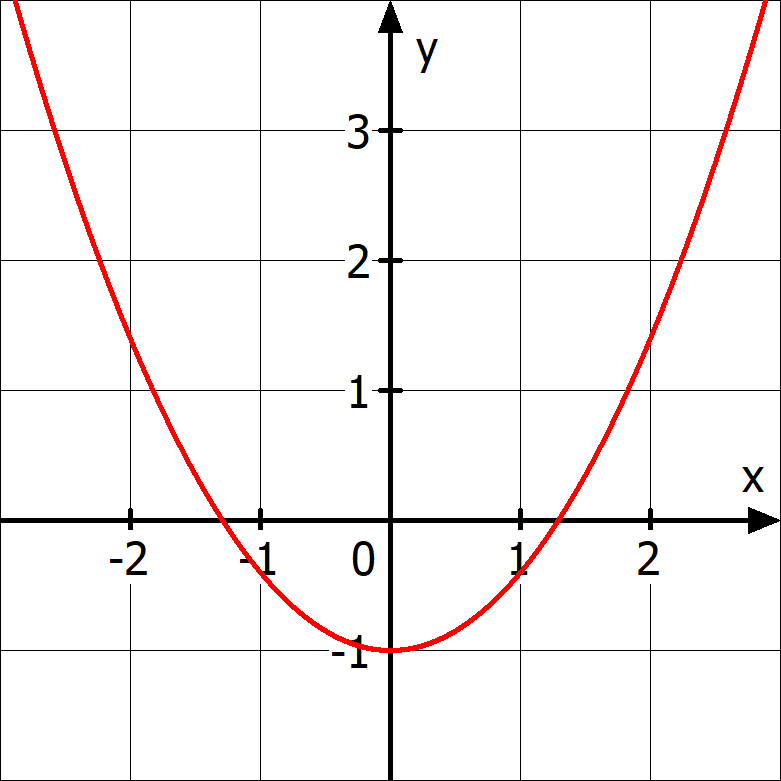
\includegraphics[width=\linewidth]{\integration/pics/Berechnen1.png}
	\end{minipage}}%
\end{minipage}

\bigskip

Das Ergebnis ist unabhängig von der verwendeten Stammfunktion:
\begin{align*}
	\int\limits_{-1}^2 \frac{3}{5}x^2-1\td x&\textcolor{loes}{\;=\left[\frac{1}{5}x^3-x+c\right]_{-1}^2=\frac{1}{5}\cdot 2^3-2+c-\left(\frac{1}{5}\cdot (-1)^3-(-1)+c\right)}\\
	&\textcolor{loes}{\;=\frac{8}{5}-2+c+\frac{1}{5}-1-c=-\frac{6}{5}}
\end{align*}

\vspace{-.5cm}

\begin{Exercise}[title={\raggedright\normalfont Berechne die Werte, der in Aufgabe \ref{integralGrafisch1} abgeschätzen Integrale, exakt.}, label=integralRechnA1]
\end{Exercise}

\vspace{-.5cm}

\begin{Exercise}[title={\raggedright\normalfont Berechne die Werte der folgenden Integrale:}, label=integralRechnA2]

	\begin{minipage}{\textwidth}
		\begin{minipage}{.5\textwidth}
			\begin{enumerate}[label=\alph*)]
				\item \(\displaystyle\int\limits_{0}^{3} 6x^2- 4\td x\)
				\item \(\displaystyle\int\limits_{0}^{1} x^3-6x^2+2 \td x\)
				\item \(\displaystyle\int\limits_{0}^{2} \frac{1}{2}x^4-\frac{3}{2}x^2+x \td x\)
				\item \(\displaystyle\int\limits_{0}^{\ln(2)} e^x \td x\)
				\item \(\displaystyle\int\limits_{0}^{2\ln(2)} -2e^{3x} \td x\)
			\end{enumerate}
		\end{minipage}%
		\begin{minipage}{.5\textwidth}
			\begin{enumerate}[label=\alph*)]
				\setcounter{enumi}{5}
				\item \(\displaystyle\int\limits_{-1}^{2} \frac{2}{3}x^2-6x+2 \td x\)
				\item \(\displaystyle\int\limits_{1}^{3} 10x^4-9x^3+4x \td x\)
				\item \(\displaystyle\int\limits_{0}^{3} 2x^2-4x \td x\)
				\item \(\displaystyle\int\limits_{-\ln(2)}^{0} -\frac{3}{2}e^{-2x} \td x\)
				\item \(\displaystyle\int\limits_{-2\ln(3)}^{2\ln(2)} -4e^{\frac{1}{2}x} \td x\)
			\end{enumerate}
		\end{minipage}%
	\end{minipage}

\end{Exercise}
%%%%%%%%%%%%%%%%%%%%%%%%%%%%%%%%%%%%%%%%%
\begin{Answer}[ref=integralRechnA1]
	\begin{enumerate}[label=\alph*)]
		\item \(\displaystyle\int\limits_{-1}^{2} -\frac{1}{4}x^3+2\td x= \frac{81}{16}\)
		\item \(\displaystyle\int\limits_{-1}^{1} -\frac{1}{4}x^3+2\td x= 4\)
		\item \(\displaystyle\int\limits_{0}^{2} -\frac{1}{4}x^3+2\td x= 3\)

		\item \(\displaystyle\int\limits_{-1}^{2} \frac{1}{3}x^2+x\td x= \frac{5}{2}\)
		\item \(\displaystyle\int\limits_{-1}^{1} \frac{1}{3}x^2+x\td x= \frac{2}{9}\)
		\item \(\displaystyle\int\limits_{0}^{2} \frac{1}{3}x^2+x\td x= \frac{26}{9}\)

		\item \(\displaystyle\int\limits_{-1}^{2} \frac{1}{10}x^3-3\td x= -\frac{69}{8}\)
		\item \(\displaystyle\int\limits_{-1}^{1} \frac{1}{10}x^3-3\td x= -6\)
		\item \(\displaystyle\int\limits_{0}^{2} \frac{1}{10}x^3-3\td x= -\frac{28}{5}\)

		\item \(\displaystyle\int\limits_{-2}^{0} -\frac{1}{5}x^4+x^2+2\td x= \frac{404}{75}\)
		\item \(\displaystyle\int\limits_{-2}^{1} -\frac{1}{5}x^4+x^2+2\td x= \frac{192}{25}\)
		\item \(\displaystyle\int\limits_{-1}^{1} -\frac{1}{5}x^4+x^2+2\td x= \frac{344}{75}\)

		\item \(\displaystyle\int\limits_{0}^{1} x^3-3x^2+\frac{1}{4}x\td x= -\frac{5}{8}\)
		\item \(\displaystyle\int\limits_{0}^{2} x^3-3x^2+\frac{1}{4}x\td x= -\frac{7}{2}\)
		\item \(\displaystyle\int\limits_{0}^{3} x^3-3x^2+\frac{1}{4}x\td x= -\frac{45}{8}\)

		\item \(\displaystyle\int\limits_{-3}^{0} -\frac{1}{3}x^2+2\td x= 3\)
		\item \(\displaystyle\int\limits_{-2}^{0} -\frac{1}{3}x^2+2\td x= \frac{28}{9}\)
		\item \(\displaystyle\int\limits_{-3}^{-2} -\frac{1}{3}x^2+2\td x= -\frac{1}{9}\)
	\end{enumerate}
\end{Answer}
\begin{Answer}[ref=integralRechnA2]
	\begin{enumerate}[label=\alph*)]
		\item \(\displaystyle\int\limits_{0}^{3} 6x^2-4 \td x=42\)
		\item \(\displaystyle\int\limits_{0}^{1} x^3-6x^2+2 \td x=\frac{1}{4}\)
		\item \(\displaystyle\int\limits_{0}^{2} \frac{1}{2}x^4-\frac{3}{2}x^2+x \td x=\frac{6}{5}\)
		\item \(\displaystyle\int\limits_{0}^{\ln(2)} e^x \td x=1\)
		\item \(\displaystyle\int\limits_{0}^{2\ln(2)} -2e^{3x} \td x=-42\)
		\item \(\displaystyle\int\limits_{-1}^{2} \frac{2}{3}x^2-6x+2 \td x=-1\)
		\item \(\displaystyle\int\limits_{1}^{3} 10x^4-9x^3+4x \td x=320\)
		\item \(\displaystyle\int\limits_{0}^{3} 2x^2-4x \td x=0\)
		\item \(\displaystyle\int\limits_{-\ln(2)}^{0} -\frac{3}{2}e^{-2x} \td x=-\frac{9}{4}\)
		\item \(\displaystyle\int\limits_{-2\ln(3)}^{2\ln(2)} -4e^{\frac{1}{2}x} \td x=-\frac{40}{3}\)
	\end{enumerate}
\end{Answer}